\documentclass[11pt,a4paper]{article}

\usepackage[margin=2.1cm]{geometry}
\usepackage{graphicx}
\usepackage{booktabs}
\usepackage{tabularx}
\usepackage{longtable}
\usepackage{array}
\usepackage{xcolor}
\usepackage{hyperref}
\usepackage{caption}
\usepackage{subcaption}

\graphicspath{{img/}}
\hypersetup{
  colorlinks=true,
  linkcolor=blue,
  urlcolor=blue
}

\newcommand{\code}[1]{\texttt{#1}}
\newcommand{\param}[1]{\texttt{#1}}
\newcolumntype{Y}{>{\raggedright\arraybackslash}X}
\newcolumntype{R}{>{\raggedleft\arraybackslash}p{0.23\linewidth}}

\title{Multi-Branch TAGE Direction Predictor\\RTL Tasarim Spesifikasyonu}
\author{}
\date{20 Agustos 2026}

\begin{document}
\maketitle

\begin{abstract}
Bu dokuman, coklu-entry TAGE yon tahmincisinin RTL seviyesinde
tasarlanabilmesi icin gerekli mikro-mimari kontrati tanimlar. Odak noktasi
tek aligned fetch-line okumasiyla ayni satirdaki birden fazla branch offset'i
icin tahmin uretilmesidir. Dokuman, simulator siniflari veya yazilim
implementasyon ayrintilari yerine tablo organizasyonu, arayuz sinyalleri,
pipeline evreleri, update kurallari, fetch-line lookup semantigi ve dogrulama
sayaclarini tarif eder.
\end{abstract}

\section{Tasarim Hedefi}

Klasik TAGE akisinda her branch PC icin ayri index/tag hesaplanir ve tablolar
branch bazinda okunur. Bu tasarimda ise fetch-line basina aligned PC ile tek
mantiksal sorgu yapilir. Her TAGE tablosunda okunan row, birden fazla entry
tasir. Her entry asagidaki alanlardan olusur:

\begin{center}
\begin{tabular}{lllll}
\toprule
\code{valid} & \code{tag} & \code{offset} & \code{ctr} & \code{u} \\
\midrule
1 bit & table'a bagli & line ici slot & saturating counter &
useful counter \\
\bottomrule
\end{tabular}
\end{center}

Fetch-line icindeki bir branch icin once actual PC'nin offset'i eslestirilir,
sonra tag karsilastirilir. En uzun history'ye sahip eslesen tagged entry
provider olur; ikinci en uzun eslesme alternate predictor olur. Provider yoksa
veya provider secilmezse tasarim bimodal tahmine duser.

\section{Parametre Seti}

Tablo~\ref{tab:core-params}, mevcut full-system deney scriptindeki varsayilan
degerleri RTL parametreleri olarak listeler. RTL tasariminda bu parametrelerin
tamami synthesis-time parameter veya CSR/config register olarak
tasarlanabilir.

\begin{table}[!htbp]
\centering
\caption{Cekirdek ve line parametreleri}
\label{tab:core-params}
\small
\begin{tabularx}{\linewidth}{@{}>{\raggedright\arraybackslash}p{0.32\linewidth}rY@{}}
\toprule
Parametre & Deger & RTL'deki anlami \\
\midrule
\param{FETCH\_WIDTH} & 4 & Bir fetch grubunda degerlendirilecek maksimum instruction sayisi. \\
\param{DECODE\_WIDTH} & 4 & Tahminci disi pipeline genisligi; valid/mask boyutlarini etkiler. \\
\param{ISSUE\_WIDTH} & 4 & Tahmin algoritmasinin parcasi degildir. \\
\param{COMMIT\_WIDTH} & 4 & Commit update port sayisini veya update FIFO bosaltma hizini etkiler. \\
\param{FETCH\_LINE\_BYTES} & 16 & TAGE aligned lookup granularity. \\
\param{MIN\_INST\_ALIGN} & 2 & RISC-V C extension icin 2-byte instruction alignment varsayimi. \\
\param{OFFSET\_WIDTH} & 3 & $\log_2(16/2)$; 16-byte line icinde 8 adet 2-byte slot. \\
\bottomrule
\end{tabularx}
\end{table}

\begin{table}[!htbp]
\centering
\caption{TAGE ve bimodal parametreleri}
\label{tab:tage-params}
\small
\begin{tabularx}{\linewidth}{@{}>{\raggedright\arraybackslash}p{0.34\linewidth}rY@{}}
\toprule
Parametre & Deger & Kullanim yeri \\
\midrule
\param{BIMODAL\_DEPTH} & 1024 & Bimodal row sayisi. \\
\param{BIMODAL\_CTRS\_PER\_ROW} & 8 & 16-byte line icindeki 2-byte slot bank sayisi. \\
\param{BIMODAL\_OFFSET\_SHIFT} & 1 & Bank seciminde byte offset'in kac bit saga kaydirilacagi. \\
\param{BIMODAL\_USE\_ALIGNED\_ADDR} & true & Bimodal row index'i aligned PC ile uretilir. \\
\param{GHISTORY\_LENGTH} & 250 & Global branch history register uzunlugu. \\
\param{PCHISTORY\_LENGTH} & 32 & Path history register uzunlugu. \\
\param{COMP\_COUNT} & 4 & Tagged TAGE tablo sayisi. \\
\param{ENTRY\_PER\_SET} & 2 & Her indexed row icindeki entry/way sayisi. \\
\param{TAG\_USE\_ALIGNED\_ADDR} & true & Tagged table tag hash'i aligned PC ile uretilir. \\
\param{PC\_HASH\_START\_FOR\_IDX} & 2 & Index PC hash baslangic biti. \\
\param{PC\_HASH\_WIDTH\_FOR\_IDX} & 10 & Index PC hash genisligi. \\
\param{PC\_HASH\_START\_FOR\_TAG} & 10 & Tag PC hash baslangic biti. \\
\param{PC\_HASH\_WIDTH\_FOR\_TAG} & 12 & Tag PC hash genisligi. \\
\bottomrule
\end{tabularx}
\end{table}

\begin{table}[!htbp]
\centering
\caption{Replacement, allocation ve history hash parametreleri}
\label{tab:alloc-params}
\small
\begin{tabularx}{\linewidth}{@{}>{\raggedright\arraybackslash}p{0.40\linewidth}rY@{}}
\toprule
Parametre & Deger & Kullanim yeri \\
\midrule
\param{HISTORY\_HASH\_TYPE} & \code{CIRCULAR\_SHIFT\_REGISTER} & Folded/CSR hash secimi. \\
\param{REPLACEMENT\_MODE} & \code{USEFUL} & Allocation kurali. \\
\param{ALLOCATE\_RANDOM\_PLACEMENT} & true & Birden fazla aday varsa LFSR ile secim. \\
\param{ALLOCATE\_LONGER\_THAN\_PROVIDER} & true & Sadece provider'dan daha uzun history'li tabloya allocate. \\
\param{PERIODIC\_RESET} & false & Useful-bit periyodik reset enable. \\
\param{PERIODIC\_RESET\_BRANCH\_PERIOD} & 262144 & Reset periodu. \\
\param{USE\_LFSR} & true & Random secim icin LFSR enable. \\
\param{LFSR\_WIDTH} & 32 & LFSR bit genisligi. \\
\param{LFSR\_SEED} & \code{0xACE1} & Reset sonrasi seed. \\
\param{LFSR\_MISPREDICTION\_UPDATE} & true & Mispredict sonrasi LFSR perturbasyonu. \\
\param{USE\_ALT\_ON\_NA} & true & Weak provider durumunda altpred secim mekanizmasi. \\
\param{NUM\_USE\_ALT\_ON\_NA} & 16 & useAltOnNA counter sayisi. \\
\param{USE\_ALT\_ON\_NA\_BITS} & 4 & useAltOnNA signed counter genisligi. \\
\param{USE\_ALT\_ON\_NA\_HASH\_START} & 2 & useAltOnNA index hash baslangici. \\
\param{USE\_ALT\_ON\_NA\_HASH\_WIDTH} & 4 & useAltOnNA index hash genisligi. \\
\bottomrule
\end{tabularx}
\end{table}

\begin{table}[!htbp]
\centering
\caption{Tagged table vektorleri}
\label{tab:table-vectors}
\small
\begin{tabular}{lrrrr}
\toprule
Alan & T0 & T1 & T2 & T3 \\
\midrule
\param{TABLE\_DEPTH} & 256 & 256 & 256 & 256 \\
\param{TABLE\_USEFUL\_WIDTH} & 2 & 2 & 2 & 2 \\
\param{TABLE\_CTR\_WIDTH} & 3 & 3 & 3 & 3 \\
\param{TABLE\_TAG\_WIDTH} & 8 & 8 & 9 & 9 \\
\param{TABLE\_HISTORY\_WIDTH} & 5 & 18 & 68 & 250 \\
\param{TABLE\_PC\_HISTORY\_START} & 0 & 0 & 0 & 0 \\
\param{TABLE\_PC\_HISTORY\_WIDTH} & 3 & 5 & 16 & 16 \\
\bottomrule
\end{tabular}
\end{table}

\section{Fiziksel Tablo Organizasyonu}

\subsection{Bimodal Tablo}

Bimodal tablo line-indexed ve banked tasarlanir:

\begin{center}
\begin{tabular}{ll}
\toprule
Yapi & \code{B[BIMODAL\_DEPTH][BIMODAL\_CTRS\_PER\_ROW]} \\
Counter & 2-bit saturating counter \\
Row index & aligned PC hash'i \\
Bank select & actual PC offset'i \\
\bottomrule
\end{tabular}
\end{center}

Varsayilan degerlerle RTL eslemesi:

\begin{quote}
\footnotesize
\begin{verbatim}
aligned_pc  = pc & ~(FETCH_LINE_BYTES - 1)
byte_off    = pc[log2(FETCH_LINE_BYTES)-1:0]
slot_off    = byte_off >> BIMODAL_OFFSET_SHIFT
bim_row     = hash(aligned_pc) % BIMODAL_DEPTH
bim_bank    = slot_off % BIMODAL_CTRS_PER_ROW
bim_pred    = B[bim_row][bim_bank].ctr[1]
\end{verbatim}
\end{quote}

Bu yapiyla 16-byte line icindeki offsetler
$0,2,4,6,8,10,12,14$ icin ayri 2-bit counter tutulur. Bu, line basina tek
bimodal row okumasiyla slot bazinda dogru counter secimini saglar.

\subsection{Tagged TAGE Tablolari}

Her component table asagidaki bicimdedir:

\begin{quote}
\footnotesize
\begin{verbatim}
T[i][TABLE_DEPTH[i]][ENTRY_PER_SET] -> Entry

Entry:
    valid  : 1 bit
    tag    : TABLE_TAG_WIDTH[i] bit
    offset : OFFSET_WIDTH bit
    ctr    : TABLE_CTR_WIDTH[i] bit
    u      : TABLE_USEFUL_WIDTH[i] bit
\end{verbatim}
\end{quote}

Offset alani byte offset degil, 2-byte slot offset olarak tasarlanir:

\begin{quote}
\footnotesize
\begin{verbatim}
offset = (pc % FETCH_LINE_BYTES) >> log2(MIN_INST_ALIGN)
       = (pc % 16) >> 1
       = 3-bit slot id
\end{verbatim}
\end{quote}

Eger bir tasarim byte offset saklamak isterse \param{OFFSET\_WIDTH}=4
olmalidir. Bu dokumanin geri kalani 3-bit slot offset varsayimini kullanir.

\section{RTL Arayuz Kontrati}

Tahminci iki mantiksal arayuze ayrilir: fetch-line prediction arayuzu ve commit
update arayuzu. Yon tahmincisi hedef adres uretmek zorunda degildir; target
ureten BTB/RAS/indirect bloklari taken biti ve PC ile ayrica beslenebilir.

\begin{table}[!htbp]
\centering
\caption{Fetch-line prediction girisleri}
\label{tab:pred-inputs}
\small
\begin{tabularx}{\linewidth}{@{}>{\raggedright\arraybackslash}p{0.28\linewidth}>{\raggedright\arraybackslash}p{0.20\linewidth}Y@{}}
\toprule
Sinyal & Genislik & Aciklama \\
\midrule
\code{pred\_req\_valid} & 1 & Yeni fetch-line tahmin istegi. \\
\code{pred\_req\_id} & impl. & Cevabi frontend ile eslemek icin sequence id. \\
\code{fetch\_pc} & XLEN & Fetch'in baslayacagi actual PC. Line ortasindan baslayabilir. \\
\code{aligned\_pc} & XLEN & \code{fetch\_pc} aligned hali; RTL icinde de hesaplanabilir. \\
\code{slot\_valid[k]} & \param{FETCH\_WIDTH} & Bu fetch grubunda decode/predecode tarafindan gecerli instruction slotlari. \\
\code{slot\_pc[k]} & XLEN & Her slotun actual PC'si. \\
\code{slot\_is\_cond[k]} & \param{FETCH\_WIDTH} & Conditional branch slotlari. \\
\code{slot\_fallthrough[k]} & XLEN & Taken degilse devam PC'si. \\
\bottomrule
\end{tabularx}
\end{table}

\begin{table}[!htbp]
\centering
\caption{Fetch-line prediction cikislari}
\label{tab:pred-outputs}
\small
\begin{tabularx}{\linewidth}{@{}>{\raggedright\arraybackslash}p{0.28\linewidth}>{\raggedright\arraybackslash}p{0.20\linewidth}Y@{}}
\toprule
Sinyal & Genislik & Aciklama \\
\midrule
\code{pred\_rsp\_valid} & 1 & Cevap valid. \\
\code{pred\_rsp\_id} & impl. & Request id geri donusu. \\
\code{slot\_pred\_valid[k]} & \param{FETCH\_WIDTH} & Slot icin yon tahmini uretildi. \\
\code{slot\_taken[k]} & \param{FETCH\_WIDTH} & Slotun predicted taken biti. \\
\code{first\_taken\_valid} & 1 & Fetch grubunda ilk taken branch var. \\
\code{first\_taken\_slot} & $\lceil \log_2(\param{FETCH\_WIDTH}) \rceil$ & Ilk taken branch slotu. \\
\code{line\_end\_history} & impl. & Bu line tahminleri uygulandiktan sonraki speculative history. \\
\code{slot\_meta[k]} & impl. & Commit update icin provider/alt/bimodal metadata kopyasi. \\
\bottomrule
\end{tabularx}
\end{table}

\begin{table}[!htbp]
\centering
\caption{Commit update girisleri}
\label{tab:update-inputs}
\small
\begin{tabularx}{\linewidth}{@{}>{\raggedright\arraybackslash}p{0.28\linewidth}>{\raggedright\arraybackslash}p{0.20\linewidth}Y@{}}
\toprule
Sinyal & Genislik & Aciklama \\
\midrule
\code{upd\_valid} & 1 & Commit veya repair update valid. \\
\code{upd\_pc} & XLEN & Branch actual PC. \\
\code{upd\_taken} & 1 & Gercek outcome. \\
\code{upd\_mispredict} & 1 & Yon tahmini yanlis veya target repair gerekli. \\
\code{upd\_is\_cond} & 1 & Conditional branch ise TAGE table update yapilir. \\
\code{upd\_meta} & impl. & Prediction cikisindaki \code{slot\_meta}. \\
\code{repair\_history} & impl. & Mispredict/squash sonrasi restore edilecek history. \\
\bottomrule
\end{tabularx}
\end{table}

\section{Pipeline Organizasyonu}

Figur~\ref{fig:model} genel veri-yolu fikrini, Figur~\ref{fig:bim} bimodal
row/bank secimini, Figur~\ref{fig:tage} ise tagged table match ve provider
secim akisini gosterir.

\begin{figure}[!htbp]
\centering
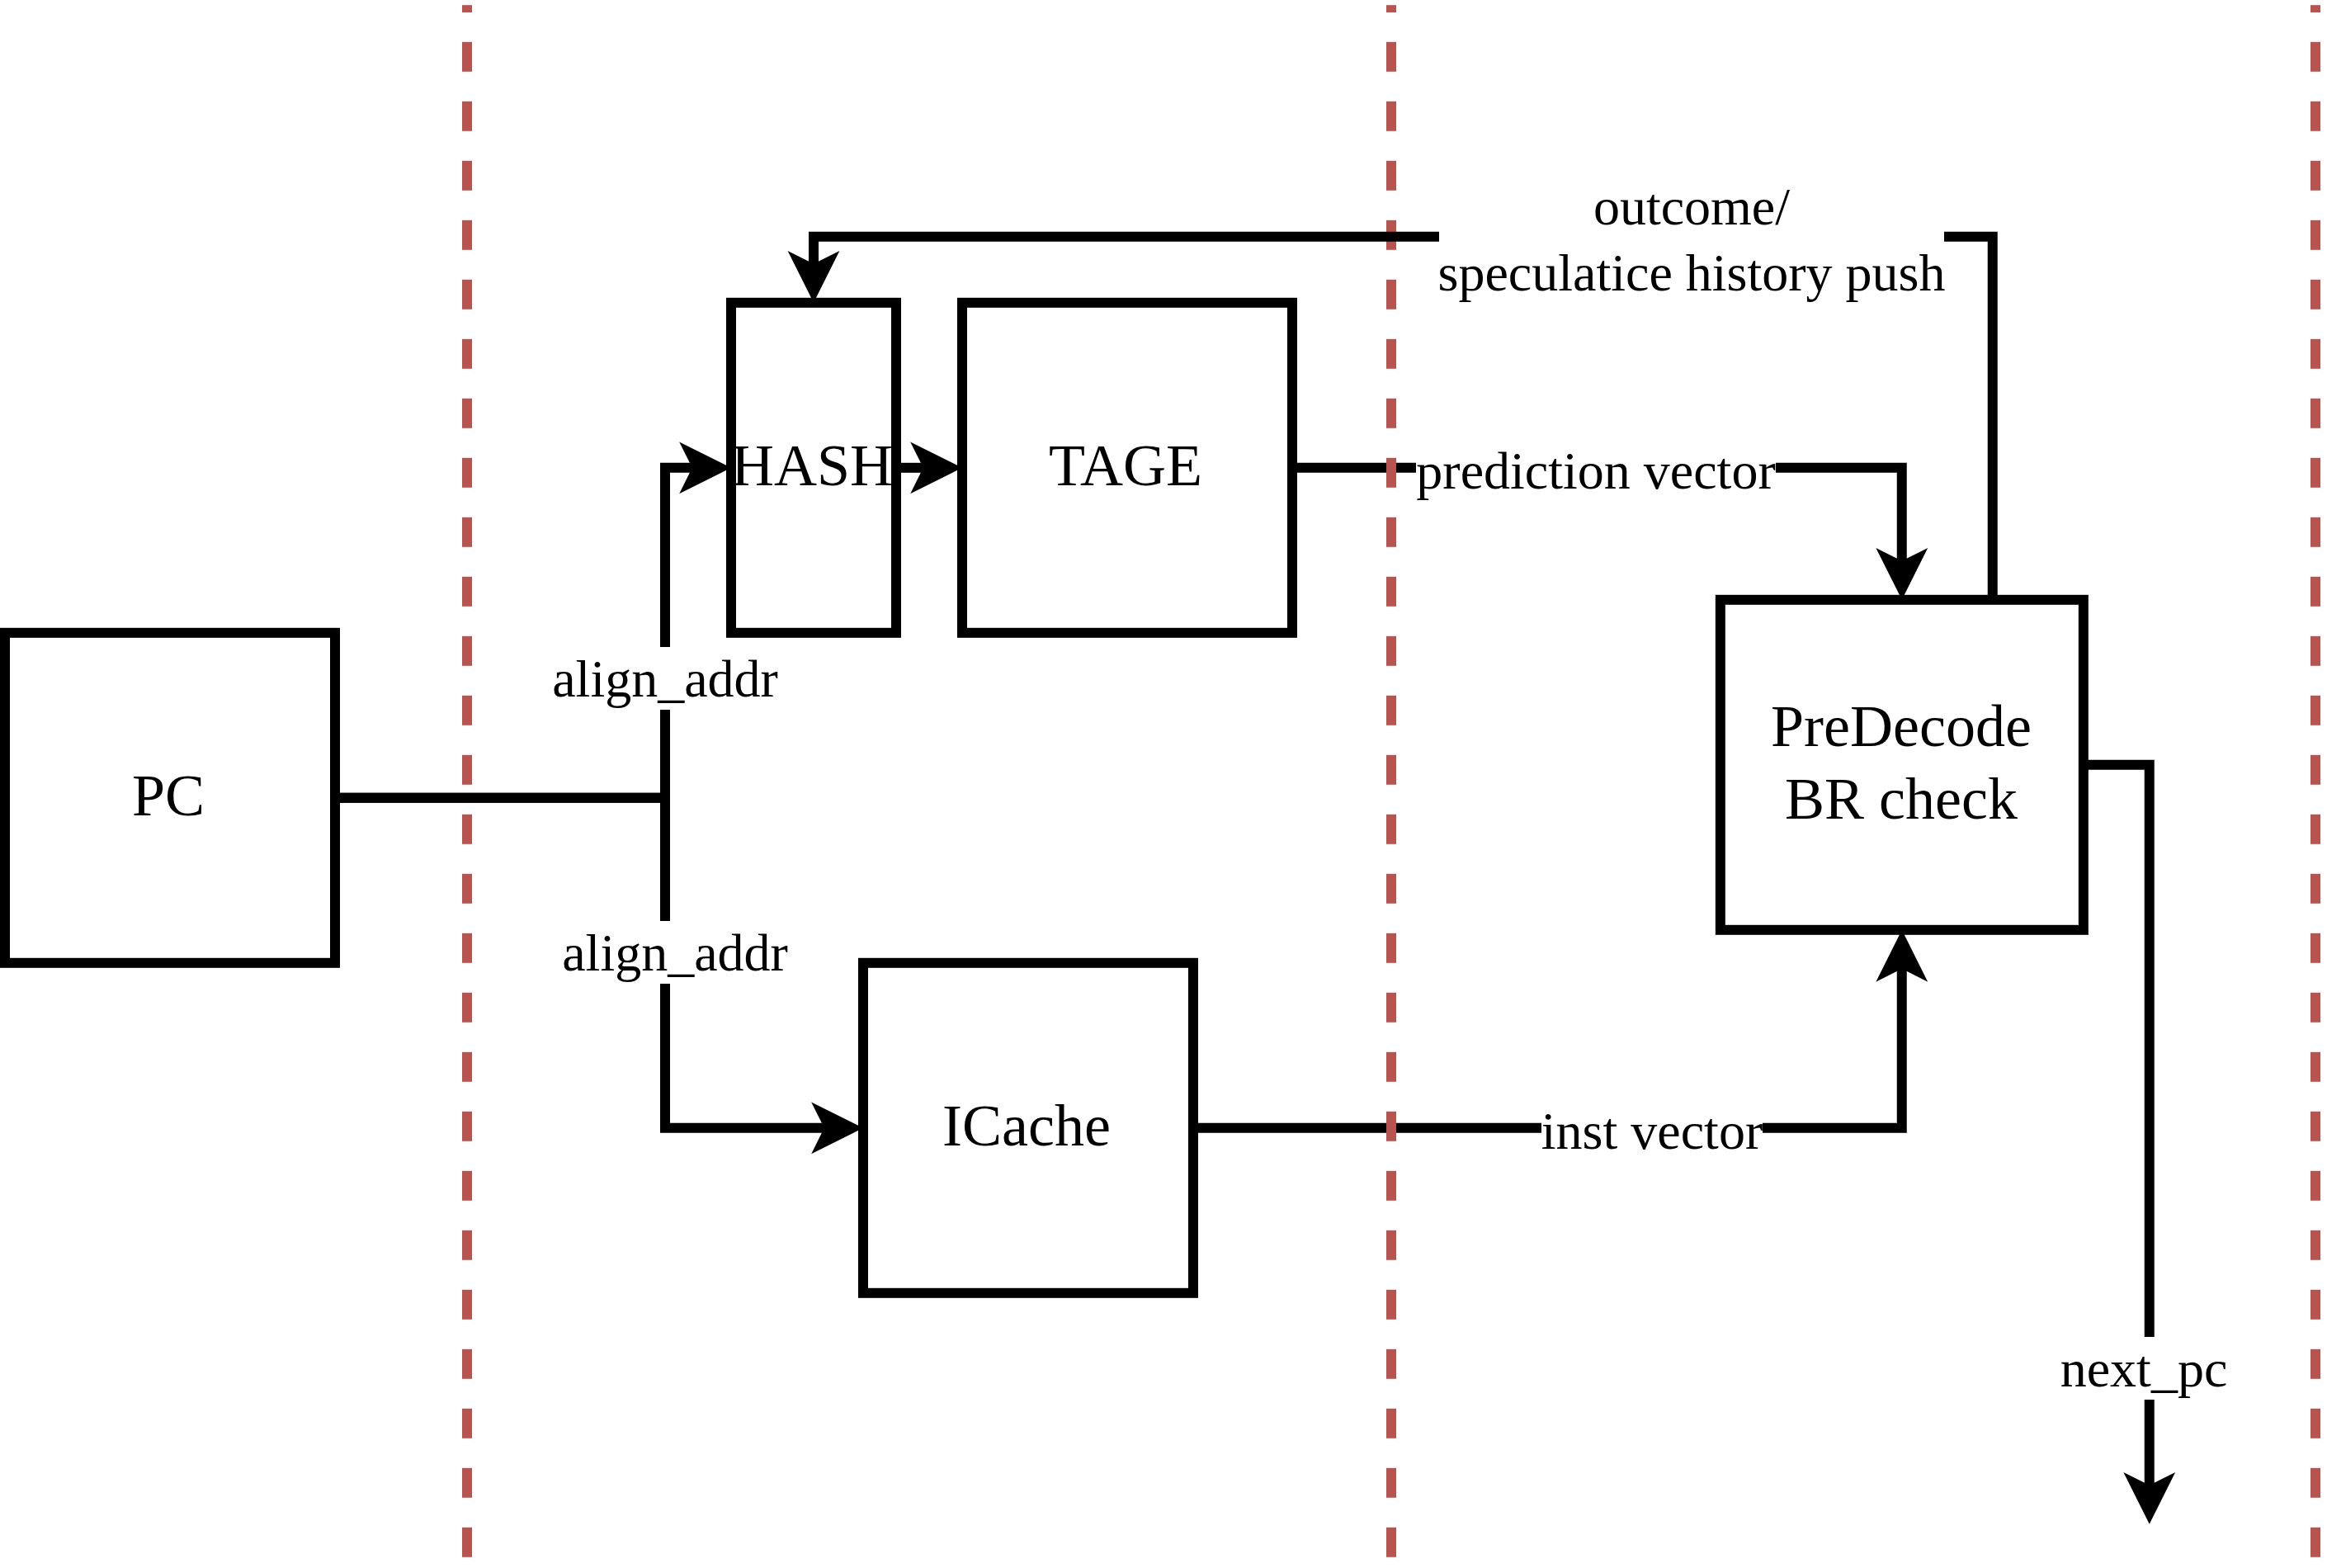
\includegraphics[width=\linewidth]{pipeline-MODEL1.drawio.png}
\caption{Multi-branch predictor genel pipeline modeli.}
\label{fig:model}
\end{figure}

\begin{figure}[!htbp]
\centering
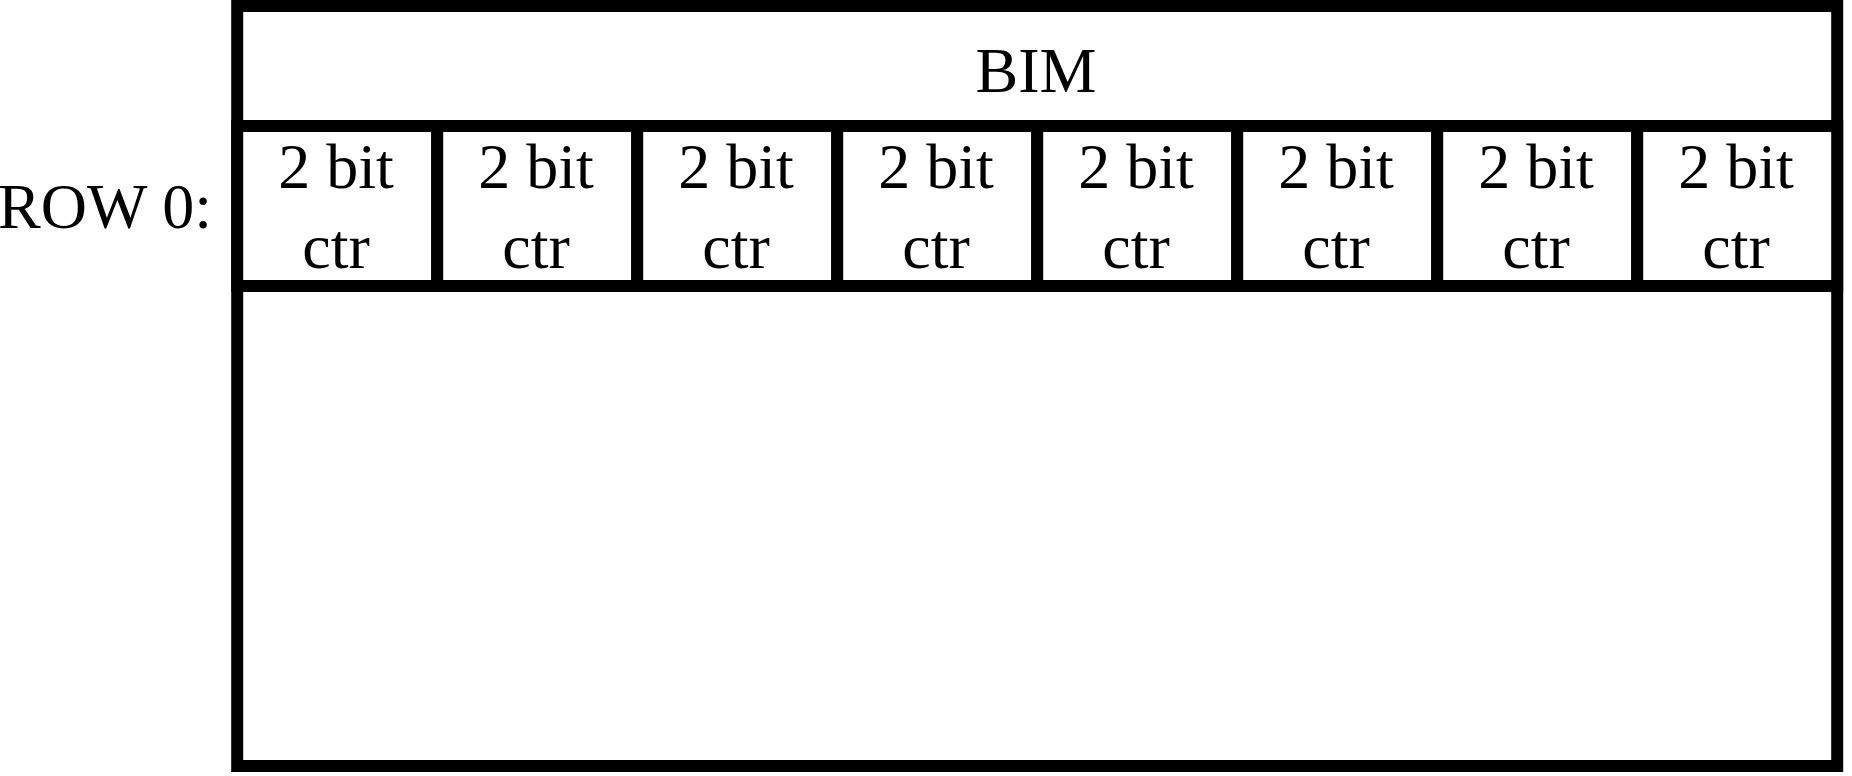
\includegraphics[width=0.95\linewidth]{pipeline-BIM.drawio.png}
\caption{Line-indexed, offset-banked bimodal tablo organizasyonu.}
\label{fig:bim}
\end{figure}

\begin{figure}[!htbp]
\centering
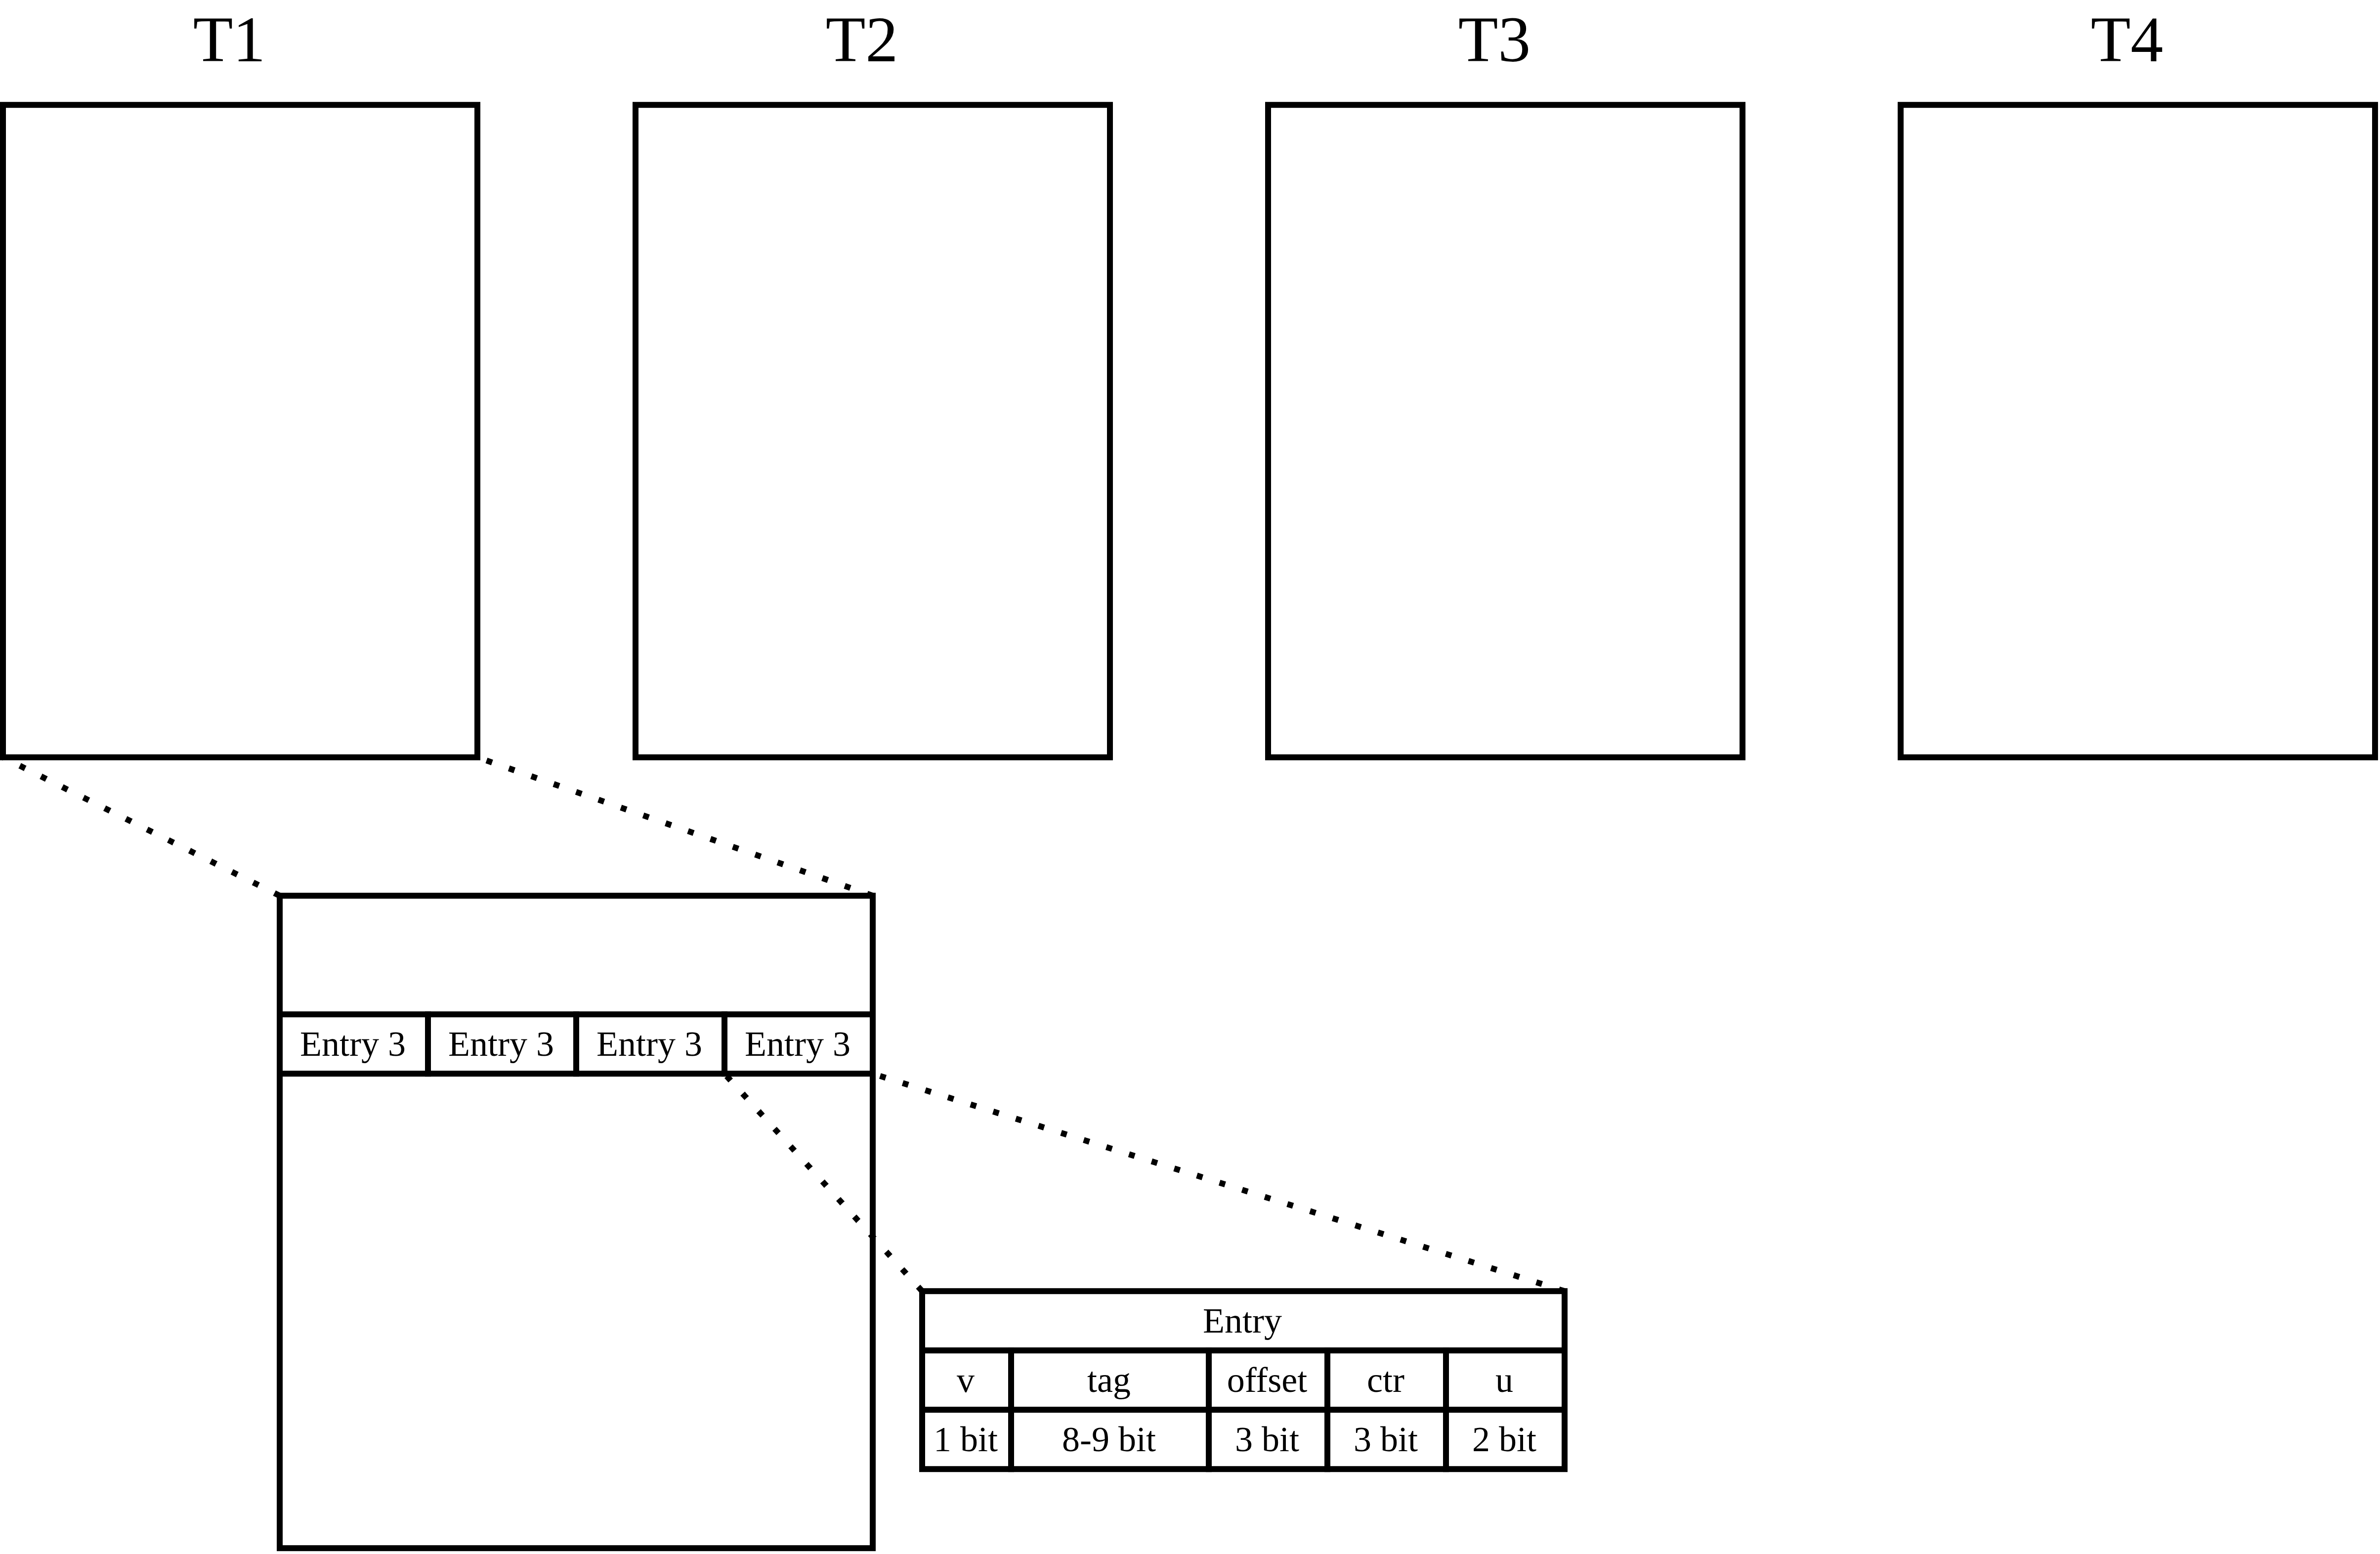
\includegraphics[width=\linewidth]{pipeline-TAGE.drawio.png}
\caption{Tagged multi-entry TAGE row okuma, offset/tag match ve provider secimi.}
\label{fig:tage}
\end{figure}

\subsection{Onerilen Evreler}

\begin{table}[!htbp]
\centering
\caption{RTL pipeline evreleri}
\label{tab:pipeline}
\small
\begin{tabularx}{\linewidth}{lll}
\toprule
Evre & Islem & Kritik cikislar \\
\midrule
P0 & Request capture, aligned PC, start slot mask & \code{aligned\_pc}, \code{active\_slot\_mask} \\
P1 & Index/tag hash, bimodal bank select & \code{idx[i]}, \code{tag[i]}, \code{bim\_row}, \code{bim\_bank[k]} \\
P2 & SRAM read: all TAGE rows and bimodal row & TAGE row vectors, bimodal counters \\
P3 & Offset CAM, tag compare, provider/alt priority & per-slot provider, altpred, fallback flags \\
P4 & useAltOnNA, final taken, first-taken priority & \code{slot\_taken[k]}, \code{first\_taken\_slot}, metadata \\
P5 & Line-end speculative history push & \code{line\_end\_history}, per-slot metadata \\
\bottomrule
\end{tabularx}
\end{table}

SRAM makrolari tek cycle read veriyorsa P2/P3/P4 ayrimi timing kapatmayi
kolaylastirir. Kucuk konfiglerde P3 ve P4 birlestirilebilir. Kritik kural:
ayni fetch-line icindeki tum slot lookup'lari ayni line-base history bit
degerleriyle hashlenir.

\section{Fetch-Line Lookup Semantigi}

Her fetch line icin once \code{aligned\_pc} uretilir. Bu \code{aligned\_pc},
tum tagged table index/tag hash'lerinde ortak PC girdisidir. Fetch line icindeki
her conditional branch icin actual PC ayrica verilir; actual PC sadece line ici
offset secimi, bimodal bank secimi ve update metadata'si icin kullanilir.

\begin{quote}
\footnotesize
\begin{verbatim}
aligned_pc = ALIGN_DOWN(fetch_pc, FETCH_LINE_BYTES)

for each conditional branch in fetch order:
    idx/tag input PC = aligned_pc
    offset input PC  = branch_pc
    pred, meta       = LOOKUP_BRANCH(aligned_pc, branch_pc,
                                     line_base_history)
\end{verbatim}
\end{quote}

Kural basittir: ayni fetch line icindeki tum branch'ler ayni
\code{aligned\_pc} ve ayni \code{line\_base\_history} ile row index/tag
hash'i uretir. Tablo satiri okunduktan sonra exact branch PC'nin offset'i ile
entry offset'i karsilastirilir. Offset bulunamazsa veya offset bulundugu halde
provider tag match yoksa sonuc bimodal yoldan gelir. Speculative history push,
tahmin sonucu uretildikten sonra frontend tarafinda program sirasiyla yapilir.

\section{Line Ortasindan Baslayan Fetch}

Fetch istegi 16-byte line basindan gelmek zorunda degildir. RTL, line basina
align ederek tablo okur ama \code{fetch\_pc}'den onceki slotlari maskeler:

\begin{quote}
\footnotesize
\begin{verbatim}
start_slot = ((fetch_pc - aligned_pc) >> log2(MIN_INST_ALIGN))

for physical slot s in 0 .. FETCH_LINE_BYTES/MIN_INST_ALIGN-1:
    before_fetch_pc = (s < start_slot)
    beyond_width    = (issued_instruction_count >= FETCH_WIDTH)
    active[s]       = slot_valid[s] && !before_fetch_pc && !beyond_width
\end{verbatim}
\end{quote}

Bu nedenle line ortasindan gelen request'te onceki instruction'lar "invalid"
edilmez; hic valid request slotu olarak islenmezler. Tahminci yalnizca
\code{active} maskesi icindeki branch'ler icin metadata ve speculative history
push eventi uretir.

\section{Prediction Pseudo-Code}

\subsection{Fetch-Line Tahmin}

\begin{quote}
\footnotesize
\begin{verbatim}
function PREDICT_LINE(fetch_pc, slots):
    aligned_pc = ALIGN_DOWN(fetch_pc, FETCH_LINE_BYTES)
    start_slot = SLOT_OFFSET(fetch_pc)
    base_hist  = current_spec_history

    for k in 0 .. FETCH_WIDTH-1:
        if !slots[k].valid or !slots[k].is_cond:
            continue
        if SLOT_OFFSET(slots[k].pc) < start_slot:
            continue

        pred, meta[k] = LOOKUP_BRANCH(aligned_pc,
                                      slots[k].pc,
                                      base_hist)

        slot_taken[k] = pred
        PUSH_SPEC_HISTORY(slots[k].pc, pred)

        if pred == TAKEN:
            first_taken_valid = true
            first_taken_slot  = k
            invalidate_younger_slots(k)
            break

    return slot_taken, first_taken_slot, meta
\end{verbatim}
\end{quote}

Buradaki \code{LOOKUP\_BRANCH} RTL pseudo-code ismidir; yazilim tarafinda bire
bir ayni isimli bir fonksiyon olmak zorunda degildir. Islevi, aligned PC ve
line-base history ile row index/tag uretmek, actual branch PC ile offset ve
bimodal bank secmek, sonra provider/altpred/bimodal kararini dondurmektir.

\subsection{Branch Lookup ve Provider Secimi}

\begin{quote}
\footnotesize
\begin{verbatim}
function LOOKUP_BRANCH(aligned_pc, branch_pc, base_hist):
    off = SLOT_OFFSET(branch_pc)

    bim_index_pc = BIMODAL_USE_ALIGNED_ADDR ? aligned_pc : branch_pc
    bim_row      = BIMODAL_ROW_INDEX(bim_index_pc)
    bim_bank     = ((branch_pc % FETCH_LINE_BYTES)
                    >> BIMODAL_OFFSET_SHIFT) % BIMODAL_CTRS_PER_ROW
    bim_ctr      = B[bim_row][bim_bank]
    bim_pred = MSB(bim_ctr)

    matches = []
    offset_match_seen = false

    for i in 0 .. COMP_COUNT-1:
        idx_i = INDEX_HASH(i, aligned_pc, base_hist)
        tag_i = TAG_HASH(i, aligned_pc, base_hist)
        row_i = T[i][idx_i]

        for way in 0 .. ENTRY_PER_SET-1:
            e = row_i[way]
            if e.valid && e.offset == off:
                offset_match_seen = true
                if e.tag == tag_i:
                    matches.push(i, way, e)

    provider = longest_history_match(matches)
    altpred  = second_longest_history_match(matches)

    if provider == NONE:
        return bim_pred, META_BIMODAL(bim_row, bim_bank,
                                      offset_match_seen)

    provider_pred = MSB(provider.ctr)
    alt_value =
        (altpred != NONE) ? MSB(altpred.ctr) : bim_pred

    weak_provider = IS_WEAK(provider.ctr, TABLE_CTR_WIDTH[provider.table])
    choose_provider = true

    if weak_provider:
        if USE_ALT_ON_NA:
            uidx = USE_ALT_INDEX(branch_pc,
                                 USE_ALT_ON_NA_HASH_START,
                                 USE_ALT_ON_NA_HASH_WIDTH,
                                 NUM_USE_ALT_ON_NA)
            choose_provider = !USE_ALT_ON_NA_PREFERS_ALT(uidx)
        else:
            choose_provider = false

    if choose_provider:
        return provider_pred, META_PROVIDER(provider, altpred,
                                           bim_row, bim_bank)
    else if altpred != NONE:
        return alt_value, META_ALTPRED(provider, altpred,
                                      bim_row, bim_bank)
    else:
        return bim_pred, META_BIMODAL_ALT(provider, bim_row, bim_bank)
\end{verbatim}
\end{quote}

\section{Commit Update Pseudo-Code}

Table training committed conditional branch stream'i uzerinden yapilir.
Speculative fetch sirasinda tablo counter'i degistirilmez; sadece speculative
history ilerletilir ve metadata FIFO'ya yazilir.

\begin{quote}
\footnotesize
\begin{verbatim}
function COMMIT_UPDATE(pc, outcome, meta):
    wrong = (meta.pred_taken != outcome)

    if USE_ALT_ON_NA && meta.has_provider && meta.provider_was_weak:
        if meta.provider_pred != meta.alt_pred:
            alt_correct = (meta.alt_pred == outcome)
            SAT_UPDATE_SIGNED(use_alt[meta.use_alt_idx],
                              alt_correct,
                              USE_ALT_ON_NA_BITS)

    if meta.has_provider:
        SAT_UPDATE(meta.provider.ctr,
                   outcome,
                   TABLE_CTR_WIDTH[meta.provider.table])

        if REPLACEMENT_MODE == USEFUL:
            if meta.provider_pred != meta.alt_pred:
                useful_inc =
                    (meta.provider_pred == outcome)
                SAT_UPDATE(meta.provider.u,
                           useful_inc,
                           TABLE_USEFUL_WIDTH[meta.provider.table])
    else:
        SAT_UPDATE(B[meta.bim_row][meta.bim_bank], outcome, 2)

    if wrong:
        ALLOCATE_ON_MISPRED(pc, outcome, meta)

    if PERIODIC_RESET:
        branch_period_counter++
        if branch_period_counter == PERIODIC_RESET_BRANCH_PERIOD:
            DECAY_OR_CLEAR_USEFUL_BITS()
            branch_period_counter = 0
\end{verbatim}
\end{quote}

\subsection{Allocation}

\begin{quote}
\footnotesize
\begin{verbatim}
function ALLOCATE_ON_MISPRED(pc, outcome, meta):
    candidates = []

    for i in 0 .. COMP_COUNT-1:
        if meta.has_provider:
            if i == meta.provider.table:
                continue
            if ALLOCATE_LONGER_THAN_PROVIDER:
                if TABLE_HISTORY_WIDTH[i] <=
                   TABLE_HISTORY_WIDTH[meta.provider.table]:
                    continue
        candidates.push(i)

    if candidates.empty:
        count_no_longer_table++
        return

    if REPLACEMENT_MODE == USEFUL:
        free_tables = []
        for i in candidates:
            if exists way in row_i with u == 0:
                free_tables.push(i)

        if free_tables.empty:
            for i in candidates:
                decrement useful bits in selected row_i
            count_no_free++
            return

        alloc_table = SELECT_TABLE(free_tables,
                                   ALLOCATE_RANDOM_PLACEMENT,
                                   USE_LFSR)
        alloc_way = FIRST_WAY_WITH_U_ZERO(alloc_table)

    else:
        alloc_table = SELECT_TABLE(candidates,
                                   ALLOCATE_RANDOM_PLACEMENT,
                                   USE_LFSR)
        alloc_way = PLRU_VICTIM(alloc_table, meta.idx[alloc_table])

    new_entry.valid  = 1
    new_entry.tag    = meta.tag[alloc_table]
    new_entry.offset = SLOT_OFFSET(pc)
    new_entry.ctr    = INIT_CTR_TOWARD(outcome,
                       TABLE_CTR_WIDTH[alloc_table])
    new_entry.u      = 0
    write T[alloc_table][meta.idx[alloc_table]][alloc_way]
\end{verbatim}
\end{quote}

\section{Hash Fonksiyonlari}

RTL implementasyonunda index ve tag hash bloklari tablo basina ayrik olabilir
veya tek paylasimli combinational bloktan pipeline register'larina yazilabilir.
CSR history hash seciminde her table icin folded history register'lari branch
history kaydikca incremental guncellenir. Index hash'inde history hash cikisi
\code{idx\_width} kadar, tag hash'inde ise \param{TABLE\_TAG\_WIDTH[i]} kadar
uretilir. Genel indeks formu:

\begin{quote}
\footnotesize
\begin{verbatim}
pc_hash_i   = bits(aligned_pc,
                   PC_HASH_START_FOR_IDX + COMP_COUNT - i,
                   PC_HASH_WIDTH_FOR_IDX)
idx_width_i = log2(TABLE_DEPTH[i])
gh_idx_hash_i =
    HISTORY_HASH(table = i,
                 history_width = TABLE_HISTORY_WIDTH[i],
                 output_width = idx_width_i)
path_hash_i = folded_path_history(TABLE_PC_HISTORY_START[i],
                                  TABLE_PC_HISTORY_WIDTH[i],
                                  output_width = idx_width_i)
idx_i       = (pc_hash_i ^ gh_idx_hash_i ^ path_hash_i)
              & (TABLE_DEPTH[i]-1)
\end{verbatim}
\end{quote}

Tag hash'i benzer sekilde uretilir:

\begin{quote}
\footnotesize
\begin{verbatim}
pc_tag_i = bits(aligned_pc,
                PC_HASH_START_FOR_TAG,
                PC_HASH_WIDTH_FOR_TAG)
gh_tag_hash_i =
    HISTORY_HASH(table = i,
                 history_width = TABLE_HISTORY_WIDTH[i],
                 output_width = TABLE_TAG_WIDTH[i])
path_tag_hash_i = folded_path_history(TABLE_PC_HISTORY_START[i],
                                      TABLE_PC_HISTORY_WIDTH[i],
                                      output_width = TABLE_TAG_WIDTH[i])
tag_i    = (pc_tag_i ^ gh_tag_hash_i ^ path_tag_hash_i)
           & ((1 << TABLE_TAG_WIDTH[i]) - 1)
\end{verbatim}
\end{quote}

Tag ve index hesaplarinda aligned PC kullanildigi icin ayni 16-byte line
icindeki farkli branch slotlari ayni row'a bakar. Offset alani bu row icindeki
hangi branch slotunun entry'yi kullanacagini secer.

\subsection{CSR History Hash}

CSR history hash, uzun global history penceresini daha kucuk bir register'a
katlayarak index ve tag hesaplarinda kullanir. Her component icin en az iki
ayri folded register tutulmasi onerilir: biri index hash'i, digeri tag hash'i
icin. Boylece table depth ve tag width farkli oldugunda her register kendi
cikis genisligine gore guncellenir.

\begin{figure}[!htbp]
\centering
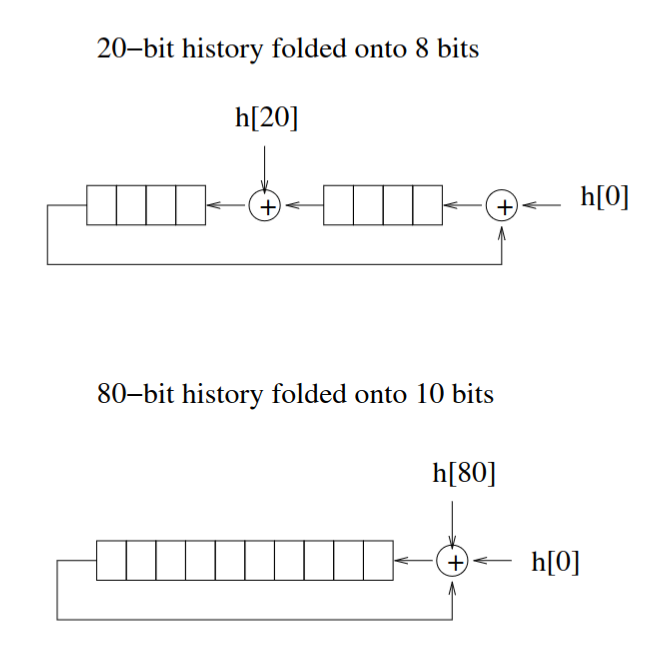
\includegraphics[width=0.52\linewidth]{CSR.png}
\caption{CSR folded history hash update mantigi.}
\label{fig:csr-history}
\end{figure}

Guncelleme denkleminde \code{C} eski folded register degeridir,
\code{C\_next} yeni folded register degeridir, \code{U} ilgili component'in
history pencere uzunlugudur ve \code{F} folded register genisligidir.
\code{new\_bit} history'ye yeni eklenen outcome bitidir. \code{old\_bit} ise
uzunlugu \code{U} olan history penceresinden disari dusen bittir.

\begin{quote}
\footnotesize
\begin{verbatim}
function CSR_UPDATE(C, U, F, new_bit, old_bit):
    tmp = C << 1

    tmp[0]     = tmp[0]     xor new_bit
    tmp[U % F] = tmp[U % F] xor old_bit
    tmp[0]     = tmp[0]     xor C[F-1]

    C_next = tmp[F-1:0]
    return C_next
\end{verbatim}
\end{quote}

Buradaki son XOR, sola kaydirma sirasinda register disina tasan
\code{C[F-1]} bitini tekrar folded alanin en dusuk bitine katlar. \code{U \% F}
terimi, history penceresinden cikan bitin folded register icindeki hangi
pozisyona katlanacagini belirler. Bu islem sayesinde uzun history penceresinin
lineer shift maliyeti yerine, her branch outcome icin sabit genislikli bir CSR
guncellemesi yeterli olur.

\begin{table}[!htbp]
\centering
\caption{Ornek tasarim icin CSR \code{U} ve \code{F} degerleri}
\label{tab:csr-uf}
\small
\begin{tabular}{lrrrrr}
\toprule
Component & $U$ & $F_{\mathrm{idx}}$ & $U \bmod F_{\mathrm{idx}}$ &
$F_{\mathrm{tag}}$ & $U \bmod F_{\mathrm{tag}}$ \\
\midrule
T0 & 5   & 8 & 5 & 8 & 5 \\
T1 & 18  & 8 & 2 & 8 & 2 \\
T2 & 68  & 8 & 4 & 9 & 5 \\
T3 & 250 & 8 & 2 & 9 & 7 \\
\bottomrule
\end{tabular}
\end{table}

Tablo~\ref{tab:csr-uf}'da $U$, \param{TABLE\_HISTORY\_WIDTH} degeridir.
Butun component'lerde \param{TABLE\_DEPTH}=256 oldugu icin index folded
register genisligi $F_{\mathrm{idx}}=\log_2(256)=8$ olur. Tag folded register
genisligi ise \param{TABLE\_TAG\_WIDTH} degerinden gelir; bu ornekte
T0/T1 icin 8 bit, T2/T3 icin 9 bittir.


\section{Storage Hesabi}

Varsayilan parametreler ve 3-bit slot offset ile kaba storage maliyeti
Tablo~\ref{tab:storage}'da verilmistir. Bu hesaba SRAM parity/ECC, valid reset
agaci, FIFO metadata, speculative checkpoint RAM ve PLRU bitleri dahil
degildir.

\begin{table}[!htbp]
\centering
\caption{Tahminci storage hesabi}
\label{tab:storage}
\small
\begin{tabular}{lrl}
\toprule
Blok & Bit & Formul \\
\midrule
Bimodal & 16,384 & $1024 \times 8 \times 2$ \\
T0 & 8,704 & $256 \times 2 \times (1+8+3+3+2)$ \\
T1 & 8,704 & $256 \times 2 \times (1+8+3+3+2)$ \\
T2 & 9,216 & $256 \times 2 \times (1+9+3+3+2)$ \\
T3 & 9,216 & $256 \times 2 \times (1+9+3+3+2)$ \\
useAltOnNA & 64 & $16 \times 4$ \\
\midrule
Toplam & 52,288 & $52,288/8 = 6,536$ byte $\approx 6.38$ KiB \\
\bottomrule
\end{tabular}
\end{table}

\section{Performans ve Debug Sayaclari}

RTL tasarimina debug icin asagidaki saturating veya wide event counter'larinin
eklenmesi onerilir. Bu sayaclar bring-up sirasinda trace modeli ve
full-system kosularla birebir karsilastirma yapmayi kolaylastirir.

\begin{table}[!htbp]
\centering
\caption{Onerilen RTL sayaclari}
\label{tab:counters}
\small
\begin{tabularx}{\linewidth}{ll}
\toprule
Sayac & Artma kosulu \\
\midrule
\code{prediction\_lookups} & Conditional branch slotu icin tahmin uretildi. \\
\code{aligned\_prediction\_lookups} & \code{aligned\_pc != slot\_pc}. \\
\code{offset\_matches} & Valid entry offset'i slot offset'iyle eslesti. \\
\code{tag\_matches} & Offset ve tag birlikte eslesti. \\
\code{provider\_found} & En az bir tagged provider bulundu. \\
\code{altpred\_found} & Provider disinda alternate tagged match bulundu. \\
\code{bimodal\_fallback\_no\_offset} & Hic offset match yok. \\
\code{bimodal\_fallback\_no\_provider} & Offset match var, tag/provider yok. \\
\code{line\_contexts\_started} & Yeni aligned fetch-line base history baslatildi. \\
\code{line\_contexts\_reused} & Ayni aligned line icin mevcut base history kullanildi. \\
\code{line\_contexts\_invalidated} & Taken tahmin, redirect veya squash line context'i kapatti. \\
\code{commit\_table\_updates} & Committed conditional branch table update'i. \\
\code{total\_allocations} & Tagged table entry allocate edildi. \\
\bottomrule
\end{tabularx}
\end{table}

\section{CoreMark 4000-Iteration Sonuclari}

Tablo~\ref{tab:terminal-results}, verilen kosunun terminal ciktisini
ozetler. Kosu resmi CoreMark skoru olarak kullanilmamalidir; cunku benchmark
10 saniye altinda bittigini raporlamistir. Predictor ve pipeline istatistikleri
ise \code{riscv-ubuntu-o3-mytage-coremark-20260820-162340-2sn-4000iter}
ROI reset/dump araligindan alinmistir.

\begin{table}[!htbp]
\centering
\caption{Terminal ciktisi ozeti}
\label{tab:terminal-results}
\small
\begin{tabularx}{\linewidth}{lY}
\toprule
Alan & Deger \\
\midrule
Komut & \code{./m5ops reset \&\& ./coremark\_nIter 4000 \&\& ./m5ops dump} \\
CoreMark size & 666 \\
Total ticks & 2,320,481 \\
Total time & 2.320481 s \\
Iterations/sec & 1723.780544 \\
Iterations & 4000 \\
Compiler & GCC 13.3.0 \\
Flags & \code{-O2 -static -march=rv64gc -mabi=lp64d -DCORE\_DEBUG=0 -lrt} \\
CRC final & \code{0x65c5} \\
Not & \code{ERROR! Must execute for at least 10 secs for a valid result!} \\
\bottomrule
\end{tabularx}
\end{table}

\begin{table}[!htbp]
\centering
\caption{ROI genel performans istatistikleri}
\label{tab:perf-results}
\small
\begin{tabular}{lr}
\toprule
Metrik & Deger \\
\midrule
Cycles & 1,996,705,225 \\
Committed instructions & 2,398,484,360 \\
IPC & 1.201221 \\
CPI & 0.832486 \\
Committed branch total & 400,750,951 \\
Committed direct conditional & 313,105,928 \\
Total branch mispredictions & 9,516,581 \\
Conditional predictions & 334,993,046 \\
Conditional predicted taken & 180,550,521 \\
Conditional incorrect & 10,923,132 \\
BTB lookups & 438,834,580 \\
BTB hits & 302,483,283 \\
BTB hit ratio & 0.689288 \\
BTB mispredicted & 4,646,677 \\
\bottomrule
\end{tabular}
\end{table}

\begin{table}[!htbp]
\centering
\caption{Multi-branch TAGE direction predictor istatistikleri}
\label{tab:mytage-results}
\small
\begin{tabular}{lr}
\toprule
Metrik & Deger \\
\midrule
Total conditional branches & 314,211,808 \\
Taken branches & 167,794,052 \\
Correct predictions & 313,392,698 \\
Miss predictions & 819,110 \\
Direction accuracy & 99.7393\% \\
Misprediction rate & 0.2607\% \\
Taken rate & 53.4016\% \\
Prediction lookups & 334,993,046 \\
Aligned prediction lookups & 303,911,512 \\
Speculative history updates & 438,834,580 \\
Commit table updates & 314,211,808 \\
Squash history restores & 38,083,631 \\
Mispredict history repairs & 10,923,132 \\
Lookup metadata records & 334,993,046 \\
History recovery records & 438,834,580 \\
Total allocations & 502,839 \\
Allocations per misprediction & 0.613885 \\
\bottomrule
\end{tabular}
\end{table}

\begin{table}[!htbp]
\centering
\caption{Selection ve match dagilimi}
\label{tab:selection-results}
\small
\begin{tabular}{lrr}
\toprule
Metrik & Count & Rate/Accuracy \\
\midrule
Bimodal selections & 198,621,258 & 63.2125\% selected, 99.9608\% acc. \\
Provider selections & 115,376,795 & 36.7194\% selected, 99.4173\% acc. \\
Alternate selections & 213,755 & 0.0680\% selected, 67.7210\% acc. \\
Offset matches & 474,383,221 & -- \\
Tag matches & 157,605,481 & -- \\
Provider found & 118,036,073 & -- \\
Altpred found & 34,385,800 & -- \\
Bimodal fallback: no offset & 80,027,026 & -- \\
Bimodal fallback: no provider & 136,929,947 & -- \\
Provider pseudo-new alloc & 376,791 & -- \\
Line contexts started & 277,212,337 & -- \\
Line contexts reused & 57,780,709 & -- \\
Line contexts invalidated & 204,367,775 & -- \\
\bottomrule
\end{tabular}
\end{table}

\begin{table}[!htbp]
\centering
\caption{Table bazli provider, altpred ve allocation sayaclari}
\label{tab:table-results}
\small
\begin{tabular}{lrrrr}
\toprule
Metrik & T0 & T1 & T2 & T3 \\
\midrule
Provider use & 46,421,726 & 48,577,226 & 10,664,355 & 9,713,488 \\
Provider hit & 46,390,475 & 48,247,670 & 10,559,910 & 9,506,430 \\
Altpred use & 34,199 & 141,563 & 37,993 & 0 \\
Altpred hit & 27,327 & 90,296 & 27,134 & 0 \\
Allocation & 4,860 & 14,503 & 75,669 & 407,807 \\
\bottomrule
\end{tabular}
\end{table}

\section{Mevcut Kod ile RTL Raporu Arasindaki Farklar}

Bu bolum, rapora gore RTL yazildiginda mevcut yazilim modelinden bilincli
olarak farkli kalacak veya birebir eslestirilmesi gereken noktalari listeler.

\begin{table}[!htbp]
\centering
\caption{Kod ve RTL spesifikasyonu karsilastirmasi}
\label{tab:code-rtl-diff}
\small
\begin{tabularx}{\linewidth}{lYY}
\toprule
Baslik & Mevcut kod davranisi & RTL raporundaki davranis \\
\midrule
Tagged offset encoding &
\code{pc\_offset(addr) = addr \% fetchLineBytes}; 16-byte line icin byte offset
saklanir ve 4 bit gerekir. &
2-byte aligned slot offset onerilir; 16-byte line icin
\code{OFFSET\_WIDTH=3}. RTL kodla bit-birebir karsilastirilacaksa byte offset
moduna alinmalidir. \\

Lookup arayuzu &
Backend lookup branch bazlidir:
\code{getPrediction(index\_addr, lookup\_addr, history\_state, state)}.
Wrapper ayni aligned line icin \code{lookupBaseState} yeniden kullanir. &
RTL arayuzu fetch-line bazlidir; line icindeki her conditional branch icin
\code{LOOKUP\_BRANCH(aligned\_pc, branch\_pc, base\_hist)} mantigi calisir. \\

History recovery &
Kodda recovery icin branch history record'lari tutulur; bunlar predictor
tablosunun algoritmik parcasi degil, recovery mekanizmasidir. &
Raporda predictor algoritmasi sadece lookup, speculative push ve commit update
olarak verilir. Recovery storage frontend/commit entegrasyonunun parcasi
olarak ele alinmalidir. \\

Bimodal row/bank &
Kodda row index \code{getIdx(index\_addr, 2, idxWidth)}, bank ise
\code{(lookup\_addr \% fetchLineBytes) >> bimodalOffsetShift}. &
Rapor ayni mantigi korur: row aligned PC'den, bank actual PC offset'inden
gelir. \\

Tag PC girdisi &
\param{TAG\_USE\_ALIGNED\_ADDR=true} iken tag hash PC girdisi aligned PC'dir. &
Rapor bu davranisi temel alir; ayni fetch line icindeki branch'ler ayni tag PC
hash girdisini kullanir. \\

CSR history hash &
Kodda index CSR genisligi \code{log2(depth)}, tag CSR genisligi
\code{tag\_width}; \code{old\_bit = global\_history[history\_width-1]}. &
Rapor ayni \code{U}/\code{F} semantigini ve \code{U \% F} insertion noktasini
tanimlar. \\

Offset/match sayaclari &
Kod \code{offsetMatches} sayacini branch basina degil, offset'i eslesen her
valid way icin artirir. &
RTL debug sayaci kodla karsilastirilacaksa ayni event tanimini kullanmalidir. \\

Counter initialization &
Bimodal counter'lar kodda weakly taken, yani 2-bit counter degeri 2 ile
baslatilir. &
RTL bring-up'ta kodla birebir eslesmek icin bimodal reset degeri weakly taken
secilmelidir. \\
\bottomrule
\end{tabularx}
\end{table}

\section{RTL Bring-Up Kontrol Listesi}

\begin{itemize}
\item Reset sonrasi tum tagged entry valid bitleri sifirlanmali, bimodal
counter'lar zayif taken veya zayif not-taken secimine gore initialize
edilmelidir.
\item 16-byte line icin \code{OFFSET\_WIDTH}=3 kullaniliyorsa sadece 2-byte
aligned PC'ler kabul edilmelidir; illegal alignment predictor request'i
uretmemelidir.
\item Ayni line icindeki iki conditional branch icin P1 index/tag hash cikislari
ayni olmalidir; sadece slot offset ve bimodal bank farkli olabilir.
\item Fetch line ortasindan baslayan request'te start slotundan onceki slotlar
metadata FIFO'ya girmemelidir.
\item Ilk predicted taken slotundan sonraki tum slotlar invalid olmalidir.
\item Commit update, prediction metadata'sindaki provider/alt/bimodal
secilimine gore ayni entry'yi guncellemelidir.
\item Mispredict repair sonrasi speculative history, recovery noktasina
donmeli; table counter update'i commit protokoluyle sinirli kalmalidir.
\item useAltOnNA counter update'i sadece weak provider ve provider/alt fikir
ayriligi durumunda yapilmalidir.
\end{itemize}

\end{document}
